% Q6 -- 4-bit data path for a processor (block diagram)
\documentclass[border=10pt]{standalone}
\usepackage{tikz}
\usetikzlibrary{arrows.meta,positioning}
\begin{document}
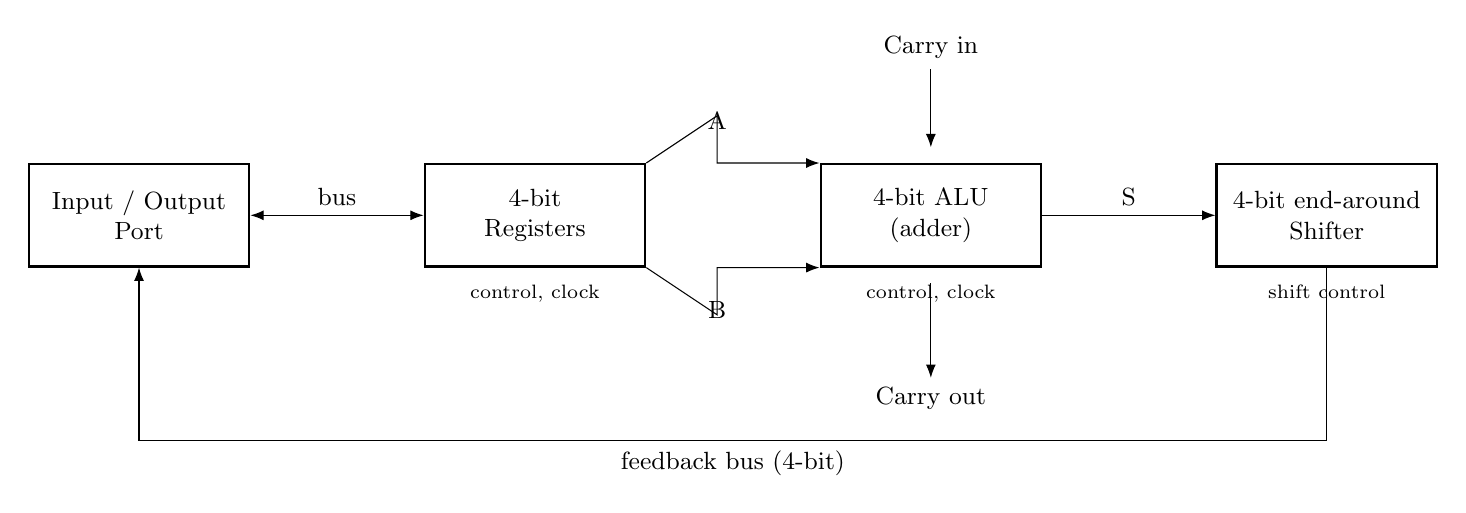
\begin{tikzpicture}[>=Latex, every node/.style={font=\small},
  blk/.style={draw, thick, minimum width=2.8cm, minimum height=1.3cm, align=center}]
\node[blk] (io)  {Input / Output\\ Port};
\node[blk, right=2.2cm of io] (reg) {4-bit\\ Registers};
\node[blk, right=2.2cm of reg] (alu) {4-bit ALU\\ (adder)};
\node[blk, right=2.2cm of alu] (sh)  {4-bit end-around\\ Shifter};
\draw[<->] (io) -- (reg) node[midway,above]{bus};
\draw[->] (reg.north east) -- ++(0.9,0.6) |- (alu.north west) node[pos=0.25,above]{A};
\draw[->] (reg.south east) -- ++(0.9,-0.6) |- (alu.south west) node[pos=0.25,below]{B};
\draw[->] (alu) -- (sh) node[midway,above]{S};
\draw[->] ([yshift=-0.2cm]alu.south) ++(0,-0.0) -- ++(0,-1.2) node[below]{Carry out};
\draw[<-] ([yshift=0.2cm]alu.north) -- ++(0,1.0) node[above]{Carry in};
% feedback bus from shifter back to I/O / registers
\draw[->] (sh.south) -- ++(0,-2.2) -| (io.south) node[pos=0.25,below]{feedback bus (4-bit)};
% control/clock hints
\node[below=0.1cm of reg, font=\scriptsize] {control, clock};
\node[below=0.1cm of alu, font=\scriptsize] {control, clock};
\node[below=0.1cm of sh,  font=\scriptsize] {shift control};
\end{tikzpicture}
\end{document}
